%!TEX root = ../dokumentation.tex

\chapter{Grundlagen}
In dem folgenden Kapitel werden die Grundlagen dieser Arbeit beschrieben. Zuerst wird das in dieser Arbeit verwendete \acs{VR}-Headset vorgestellt. Nach dem \acs{VR}-Headset folgt der Eye Tracker und zum Schluss die Laufzeit- und Entwicklungsumgebung Unity.

\section{\acl{VR}}
Der Begriff \ac{VR} oder Virtuelle Realität ist eine Technik, die beschreibt wie 

\section{\acs{VR}-Headset}
Im Rahmen dieser Arbeit wird das \acs{VR}-Headset HTC Vive verwendet. Das Headset wurde gemeinsam von den Firmen HTC und Valve entwickelt. Das \acs{VR}-Headset lässt sich in die folgenden 3 Teile unterteilen. 

\cite{Clay_Koenig_Koenig_2019}
\subsection{\acl{HMD}}
Das \ac{HMD} ist 
\todo{Abbildung von Headset}

\subsection{Controller}
\todo{Abbildung von Controller}

\subsection{Lighthouse Tracking System}
\todo{Abbildung von Basisstation}

\section{Eyetracking}
Eyetracking ist eine Technologie, die erkennt, in welche Richtung eine Person ihren Blick richtet. Hierfür werden beim Eyetracking Blick sowie Augenbewegungen erfasst. Die hauptsächlichen Parameter, die durch das Eyetracking erfasst werden, sind Fixiationen (von dem Benutzer fixierter Punkt oder Objekt), Sakkaden (schnelle Augenbewegungen bei der Erfassung eines neuen Fixpunktes) und Regression (Rücksprung zu vorherigen Fixpunkte oder Objekte).

\begin{figure}[!htbp]
	\centering
	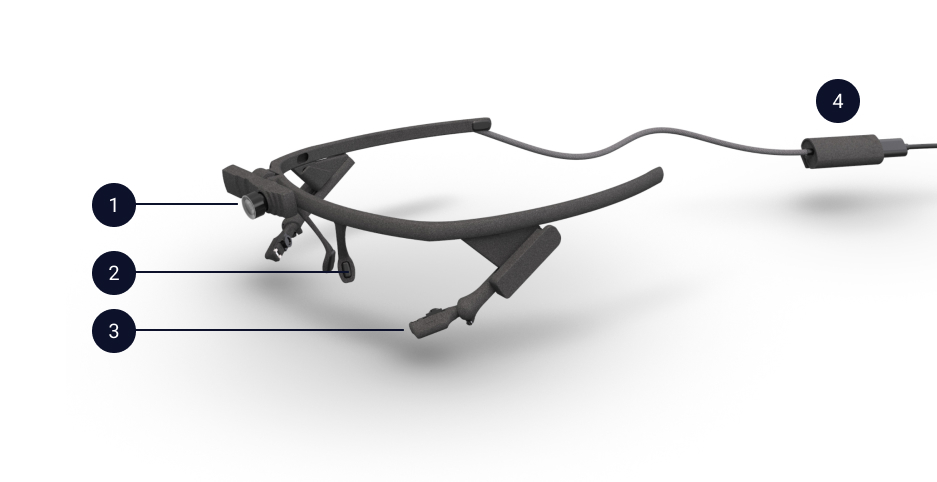
\includegraphics[width=1\linewidth]{pupil_labs_headset}
	\caption{Pupil Core Headset}
	\label{fig:pupil_labs_headset}
\end{figure}

\todo{Quelle aus Pupil Labs Dokumentation --> Core --> Hardware}

Im Rahmen dieser Arbeit wird ein Eyetracker von Pupil Labs verwendet. Sie entwickeln seit 2014 die Plattform Pupil Core, die aus einer Open-Soure-Suite sowie dem Eyetracker selber besteht. In \autoref{fig:pupil_labs_headset} ist das tragbare Eyetracker Headset Pupil Core zu sehen, welches wie eine Brille getragen wird. An dem Headset ist eine Blickfeldkamera (Nummer 1) angebracht, welche das Blickfeld des Benutzers aufnimmt. Mithilfe der Augenkameras (Nummer 3) lässt sich das komplette Auge erfassen. Die Augenkameras lassen sich individuell auf die Augen einstellen. Ein USB-C Kabel (Nummer 4) dient als Stromversorgung sowie für den Austausch der Videodaten der Kameras. Wird der Eyetracker mit dem Computer verbunden, dann lässt sich mit der Pupil Core Software das Eyetracking starten. Mithilfe der Software lassen sich die Eyetracking-Daten aus den Videostreams auslesen, auswerten und über eine Netzwerk Schnittstelle zur Verfügung stellen. Zudem kann in das Umgebungsvideo der Blickfeldkamera der Punkt angezeigt werden, auf den der Benutzer seinen Blick fixiert. \\
Da in dieser Arbeit das Eyetracking innerhalb einer \ac{VR}-Umgebung untersucht werden soll, wird ein speziell für die HTC Vive entwickelter Eyetracker von Pupil Labs verwendet. Dies ist ein Add-on von Pupil Labs, welches in das HTC Vive Headset eingebaut wird und während dem Tragen des Headsets verwendet werden kann.

\todo{Bild von Add-on hinzufügen}

\cite{PaperPupilLabs}

\section{Unity}

\subsection{steamVR}

\subsection{hmd\_eyes}